%Andrzej told us to reduce the size of the Future Work because it is way too large. I commented  some sentences of minor importance. 
\subsection{Collections}\label{subsec:collections}
When managing even more complex buildings, it might be necessary to have collections of instances. This could be simple arrays, lists or something like the generics of java. It might prove difficult to convey the concept to non-programmers, so the actual syntax should be defined together with future users.

\subsection{Graphical Editor for policy definition}\label{subsec:graphicaleditor}
Our DSL editor is text based and we have decided to use concepts and words commonly used in the industry. In the way they are structured and used in our DSL, they literally describe the meaning of the combined keywords. However, one needs to have some programming knowledge in order to understand and know how to use the expression language. Therefore, our DSL could be improved by developing a graphical editor for the policies to abstract the expression language and consequently make it simpler for users to define them.

\subsection{Integration with existing systems}\label{subsec:integration}
In our metamodel, we have included some external systems that already exist; (\textit{CTS, Access Control, Calender System and Meeting Schedule Systems}) and used in some buildings. Those systems are usually closed, proprietary systems and therefore fall outside the scope of this paper. Some form of integration is possible to some of them, but would need to be evaluated case by case. For instance, (\textit{CTS}) is somewhat advanced and needs thorough knowledge of the tool to properly use it. 
\begin{comment}The GUI looks like an electrical diagram, and is not made for ease of use. Moreover, the temperatures shown in the program are from sensors in the ventilation ducts, not in the room themselves, adding extra complexity. 
\end{comment}
As it is today, it is not really possible to integrate CTS systems into custom made solutions, like our DSL, since they are proprietary systems and guarded well in order to sell service packages to the users.

\subsection{Enhanced Code Completion}\label{subsec:codecompletion}
Code completion is of great importance to our language because it really helps the user by guiding her in all possible options she has. Right now our DSL has an up-and-running code completion but in the future we would like to restrict it in a way that only the declared/defined elements should be available. In \nameref{fig:code-completion} below, we present our DSL as it currently is but if restricted, should only be able to provide TemperatureSensor and RadiatorActuator as options for the TemperatureControlPolicy to the user.

%Andrzej told us to remove this figure totally
\begin{comment}
\begin{figure}
  \centering
    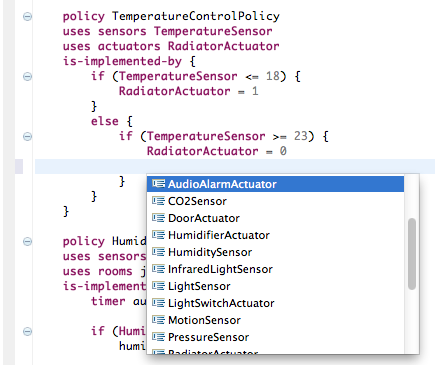
\includegraphics[scale=.5]{dsl-code-completion.png} 
	\caption{An example of \textit{code completion}.}
	\label{fig:code-completion}
\end{figure}

%This point has been recently implemented!
\subsection{Defining Actuator and Sensor types}\label{subsec:def-sensor-actuator-types}
From the evaluation section above, we came to realize that some of the sensors and actuators needed to satisfy the requirements are not implemented in our DSL. A quick fix would be to add them to our metamodel but this still will not give us the flexibility to define policies using actuators and sensors that are not available in our DSL when needed. Future work in this area might include a minor modification of our DSL in order to accommodate definition of actuators and sensors as needed. Sort of the same concept as the predefined room types. This flexibility will make our DSL more adaptable.
\end{comment}

\subsection{Prioritization}\label{subsec:looptime}
Prioritization of policies would be nice to have in a future version of our language. For example, higher priorities could be given to policies handling situations concerning fire alarms. At the moment we imagine the DSL running in a loop that calls all active (determined using the \textit{schedules}) policies in every iteration. This could instead be based on a prioritization of room, room-type or policies adding extra flexibility and fine grained control to the language. For instance, specify that some policies should only run once in an hour, and some should be run so fast that handling of for example fire alarms would happen almost instantaneous. 

\subsection{When to run policies}\label{subsec:during}
In its current state, our DSL allows us to determine when the policies should be run by using the already defined schedules. One or more policies can be run based on one or more schedules. As shown in the image below, we specify a schedule for all governing policies of that room-type. 
\begin{figure}
  \centering
    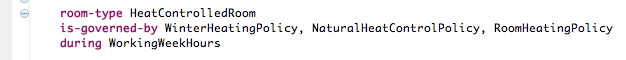
\includegraphics[scale=0.5]{dsl-during.png} 
	\caption{An example showing how to chain together policies with execution schedules using the \textit{during} keyword.}
	\label{fig:during}
\end{figure}
In case we have several governing policies that run on different schedules, our DSL does not allow us to assign a specific schedule to every single governing policy. An interesting improvement that could increase our DSL's flexibility would be the ability to specify a different schedule for each of the policies governing a room.